\chapter{Results}
In this chapter, we have represented numerical and graphical results of fall detection. Here, We have found fused dataset using both UR dataset and Open labeled dataset which have been preprocessed to extract features gives more accuracy than the individual one to detect a fall. 

\section{Numerical Analysis}
% This section discussed the numerical results obtained using state-of-the-art classifiers. We have utilized Weka for evaluating the performance of the classification algorithms (RF, SVM, and RNN) which can be used to detect falls as well as the normal daily activities of the people with neurological diseases.  For each classifier, we use precision, sensitivity, specificity, and F-1 score. 

The numerical results obtained using state-of-the-art classifiers have been addressed in this section. Weka was used to evaluate the efficiency of the classification algorithms (RF, SVM, and RNN) that can be used to diagnose crashes, as well as the normal everyday behaviors of persons with neurological diseases. 

\vspace{.5cm}

Weka is a highly effective open source machine learning framework that can be managed through a gui, conventional terminal uses, or a Java API. It is extensively used for training, screening, and commercial uses, offers a wealth of built-in tools for conventional machine learning operations, and allows direct access to well-known toolkits such as For any classification algorithm, we utilize accuracy, sensitivity, specificity, and F-1 score.


% Weka is tested and proven platform for open source machine learning that can be controlled through a graphical user interface, traditional terminal applications, or a Java API. It is commonly used for training, testing, and industrial applications, includes a plethora of built-in resources for standard machine learning activities and also provides straightforward access to well-known toolkits such as sci-kit-learn, sci-kit-learn. We use consistency, sensitivity, specificity, and F-1 score for each classifier.

\vspace{.5cm}
The suggested fall detection architecture based on RNN contains two parallel structures, each consisting of a layer of batch normalization, an RNN layer, and a fully connected layer followed by layers of softmax output. The model was trained on the training dataset using the Adam optimizer and for 30 epochs with a learning rate of 0.001, a batch size of 32 and an RNN dropout of zero. After preparation, a different research dataset was used to test the model.

% The proposed RNN based fall detection architecture contains two parallel structure, each consists of a batch normalization layer, an RNN layer and a fully-connected layer followed by softmax output layers. The model was trained using Adam optimizer and for 30 epochs with a learning rate of 0.001, batch size of 32 and RNN dropout of zero on the training dataset. After training, the model was tested using the separated test dataset.

\vspace{.5cm}
Table \ref{resulttab:2} shows the classification performance of RF, SVM and RNN.

\begin{table}[!ht]
    \centering
     \scriptsize
    \begin{tabular}{lcccccc}
    \toprule
      Dataset &Classifier& Accuracy& Precision&Sensitivity&Specificity&F1-Score \\\cmidrule{1-7}
        Open Labelled&RF & 0.96801&0.95979&0.98411&0.94749 & 0.97179\\ \cmidrule{2-7}
          &SVM  &0.98101 &0.9754&0.99139&0.96752&0.98333\\\cmidrule{2-7}
           & RNN  &0.97226&0.96369 & 0.98711&0.95257&0.97555 \\ \midrule
        URRF & RF &0.95652&0.96296&0.96296&0.94737&0.96296 \\ \cmidrule{2-7}
          &SVM  &0.97778	 &0.96296	&1	&0.94737&0.98113	\\\cmidrule{2-7}
           & RNN  &0.95652 &0.96428& 0.96429&0.94444&0.96429 \\\midrule
          Fused&RF &0.9680 &0.9598&0.9841&0.9475&0.9718 \\ \cmidrule{2-7}
          &SVM  &0.9808 &0.97506&0.9913&0.9675&0.9831\\\cmidrule{2-7}
           & RNN  &0.9723 &0.9637& 0.9877&0.9526&0.9756 \\\bottomrule
             		
    \end{tabular}
    \caption{Performance comparison of RNN with RF and SVM}
    \label{resulttab:2}
\end{table}

\vspace{.5cm}
From the table (see table \ref{resulttab:2}) that RNN and SVM have higher precision, accuracy, specificity and F1-Score than RF. In RF, however, the sensitivity is higher than in SVM and RNN. We can see from an overall study that the Fused algorithm offers better precision, accuracy, sensitivity, specificity, and F1-score, whereas the Open label gives the lowest value of these output matrices.

% From the table (see table \ref{resulttab:2}), we can depicted that RNN and SVM have better accuracy, Precision, specificity and F1-Score than the RF. But the sensitivity is better in RF then the SVM and RNN. From overall analysis, we can see that the Fused algorithm gives better Accuracy, precision, sensitivity, specificity, and F1-score, whereas Open labelled gives the lowest value of these performance matrices.
\section{Graphical Analysis}
 Graphical Analysis of Open Labelled, URRF and Fused dataset to detect fall have been represented in this section. Here, We have used bar charts to compare accuracy, precision, sensitivity, specificity, f1 score among the classifiers RF, SVM, RNN.
 
 \vspace{0.5cm}
Figure \ref{fig:Chart 1} shows the accuracy, precision, sensitivity, specificity and F1 score level of Open labelled algorithm. We can see that SVM, RF and RNN give exellent result and the result is quite similar. But in every level SVM give better result among of them. 
\begin{figure}[!ht]
    \centering
    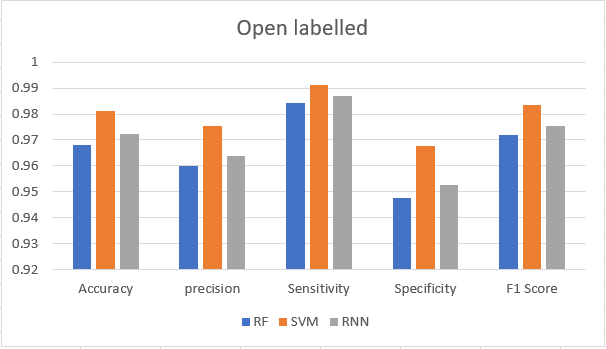
\includegraphics[scale=0.75]{Chap5/Bar 1.PNG}
    \caption{Graphical Analysis of Open Labelled dataset}
    \label{fig:Chart 1}
\end{figure}

\vspace{0.5cm}
In URRF algorithm (see figure \ref{fig:Chart 2})the results differ. Series 1 is better than series 2 and 3 in accuracy, sensitivity and F1 score level but in precision and speciality level both series 1 and series 2 gives quite similar output and series 3 gives better precision. 
\begin{figure}[!ht]
    \centering
    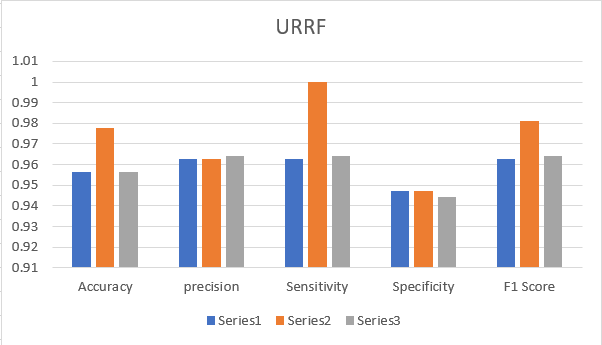
\includegraphics[scale=0.75]{Chap5/Bar 2.PNG}
    \caption{Graphical Analysis of URRF dataset}
    \label{fig:Chart 2}
\end{figure}

Figure \ref{fig:Chart 3} shows the accuracy, precision, sensitivity, specificity and F1 score level of fused algorithm. We can see that SVM, RF and RNN give exellent result and the result is quite similar. But in every level SVM give better result among of them.  
\begin{figure}[!ht]
    \centering
    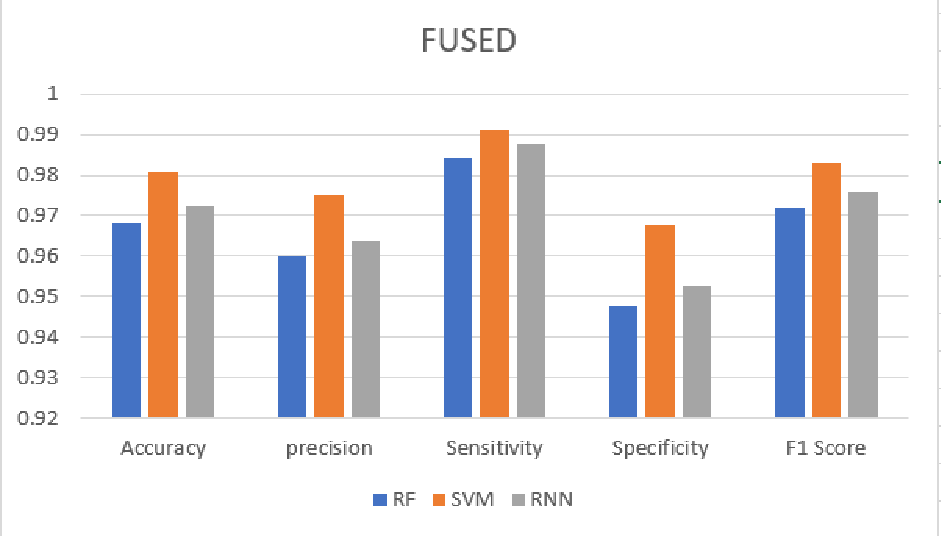
\includegraphics[scale=0.67]{Chap5/Bar.pdf}
    \caption{Overall Analysis of fused Algorithm through Bar Chart}
    \label{fig:Chart 3}
\end{figure}





% \vspace{0.5cm}
% Fig \ref{fig:Chart 3} shows the accuracy, precision, sensitivity, specificity and F1 score level of fused algorithm. We can see that SVM, RF and RNN give exellent result and the result is quite similar. But in every level SVM give better result among of them.  